\documentclass[tikz, border=10pt]{standalone}
\usetikzlibrary{calc}

\begin{document}
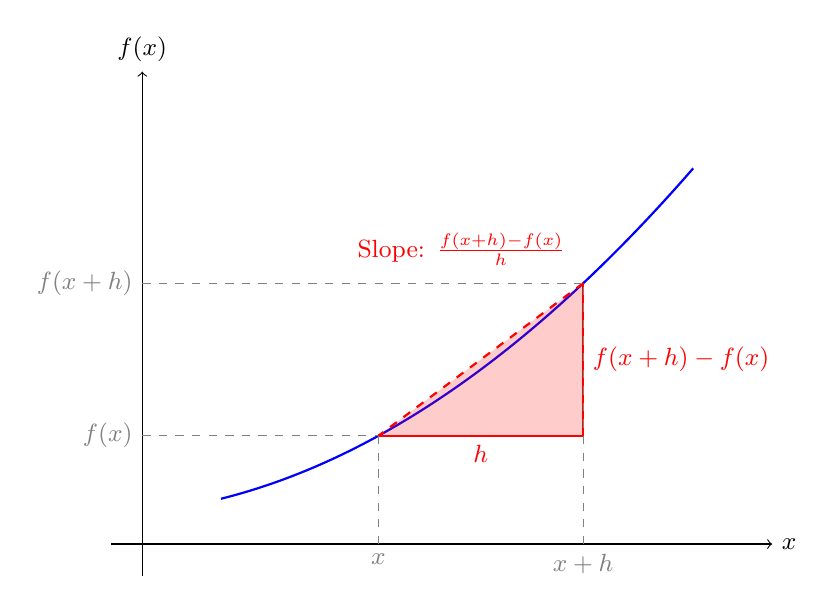
\begin{tikzpicture}[
    scale=2.0,
    important line/.style={thick},
    dashed line/.style={dashed, thin, gray},
    every node/.style={font=\small},
    triangle fill/.style={fill=red, fill opacity=0.2}, % Translucent fill
    triangle stroke/.style={red, thick}
]
    % Axes
    \draw[->] (-0.2,0) -- (4,0) node[right] {$x$};
    \draw[->] (0,-0.2) -- (0,3) node[above] {$f(x)$};

    % Curve
    \draw[important line, blue] plot[domain=0.5:3.5, samples=100] (\x, {0.15*\x*\x + 0.1*\x + 0.2});
    
    % Definitions
    \def\xval{1.5}
    \def\hval{1.3}
    \def\xphval{2.8}
    \pgfmathsetmacro{\fx}{0.15*\xval*\xval + 0.1*\xval + 0.2}
    \pgfmathsetmacro{\fxph}{0.15*\xphval*\xphval + 0.1*\xphval + 0.2}

    \coordinate (P) at (\xval, \fx);
    \coordinate (Q) at (\xphval, \fx);
    \coordinate (R) at (\xphval, \fxph);

    % Translucent Triangle
    \fill[triangle fill] (P) -- (Q) -- (R) -- cycle;
    \draw[triangle stroke] (P) -- (Q); 
    \draw[triangle stroke] (Q) -- (R); 
    \draw[triangle stroke, dashed] (R) -- (P); 

    % Adjusted Labels
    \path (P) -- (Q) node[midway, below, red] {$h$};
    \path (Q) -- (R) node[midway, right, red] {$f(x+h) - f(x)$};
    
    % Moved slope text to the left and up to avoid overlap
    \node[red, anchor=south east, xshift=-0.1cm, yshift=0.1cm] at (R) {Slope: $\frac{f(x+h)-f(x)}{h}$};

    % Projections
    \draw[dashed line] (\xval,0) node[below] {$x$} -- (P);
    \draw[dashed line] (\xphval,0) node[below] {$x+h$} -- (R);
    \draw[dashed line] (0,\fx) node[left] {$f(x)$} -- (P);
    \draw[dashed line] (0,\fxph) node[left] {$f(x+h)$} -- (R);
\end{tikzpicture}
\end{document}